\documentclass[12pt,a4paper]{report}
\usepackage[utf8]{inputenc}
\usepackage{graphicx}
\usepackage{hyperref}
\usepackage{geometry}
\usepackage{booktabs}
\usepackage{titlesec}
\usepackage{tikz}
\usetikzlibrary{shapes.geometric, arrows, positioning, fit, calc}

\geometry{a4paper, margin=1in}

\titleformat{\chapter}[display]
  {\normalfont\huge\bfseries}{\chaptertitlename\ \thechapter}{20pt}{\Huge}
\titlespacing*{\chapter}{0pt}{50pt}{40pt}

\begin{document}

\begin{titlepage}
    \centering
    \vspace*{2cm}
    
    {\Large Software Engineering Project Report \par}
    \vspace{1.5cm}
    
    {\Huge\bfseries MathVerse AI \par}
    \vspace{0.5cm}
    {\Large \textit{Frontend Prototype and User Interface Implementation} \par}
    
    \vspace{3cm}
    
    {\Large \textbf{Submitted by:} \par}
    Your Name (Roll Number) \par
    Team Member 2 (Roll Number) \par
    \vspace{1.5cm}
    
    {\Large \textbf{Submitted to:} \par}
    Professor / Evaluator Name \par
    
    \vfill
    
    {\Large \textbf{Mid-Semester Evaluation} \par}
    {\Large \textbf{Computer Science and Engineering Department} \par}
    {\Large Thapar Institute of Engineering and Technology, Patiala \par}
    \vspace{1cm}
    
    {\large \today \par}
\end{titlepage}

\tableofcontents
\newpage

\chapter{Introduction}

\section{Background and Context}
Mathematics anxiety and a lack of student engagement are pervasive challenges in modern education. Traditional pedagogical methods often fail to motivate students. MathVerse AI seeks to solve this by creating an immersive, gamified learning platform that combines superhero-themed narrative elements (such as "Boss Battles" and "Missions") with an interactive user experience. This report details the work completed during the initial prototype phase, which focuses entirely on the design, architecture, and implementation of the Frontend User Interface.

\subsection{Problem Statement}
Before integrating complex backend services and Artificial Intelligence models, the project required a robust, highly responsive, and engaging user interface. The primary challenge was translating gamified concepts—such as tracking "Spider Points," visualizing health bars during boss battles, and navigating interactive missions—into a seamless web application that performs fluidly across devices without overwhelming the user.

\section{Project Objectives (Prototype Phase)}
\begin{enumerate}
    \item \textbf{Objective 1:} Design and implement a responsive, modern web application frontend using React 18, Vite, and Tailwind CSS.
    \item \textbf{Objective 2:} Develop reusable, interactive UI components for core gamification features, including \texttt{BossBattles}, \texttt{Missions}, and \texttt{Gamification} dashboards.
    \item \textbf{Objective 3:} Establish a robust client-side state management architecture to track user progress, health points, and virtual currency locally before backend integration.
    \item \textbf{Objective 4:} Ensure high fidelity in animations and transitions (using specialized components like \texttt{Reveal.tsx}) to reinforce the superhero thematic experience.
\end{enumerate}

\chapter{Methodology and Design}

\section{System Architecture}
The work completed thus far constitutes the Presentation Layer (Frontend) of the MathVerse AI platform. It is built as a Single Page Application (SPA) to ensure rapid navigation without page reloads, maintaining the immersive "game-like" feel of the platform.

\subsection{High-Level Design}
The frontend architecture is modular, splitting the application into distinct feature-based components. The landing experience comprises the \texttt{Hero}, \texttt{HowItWorks}, and \texttt{Testimonials} components. Once authenticated (currently mocked), the user interacts primarily with the \texttt{Dashboard}, which acts as the central hub for accessing \texttt{Missions} and \texttt{BossBattles}. The \texttt{MissionPlayer} component governs the active learning state, presenting mathematical challenges to the user.

\subsection{Technical Stack}
\begin{itemize}
    \item \textbf{Core Framework:} React 18 with TypeScript for static type safety.
    \item \textbf{Build Tool:} Vite, providing extremely fast Hot Module Replacement (HMR) and optimized production builds.
    \item \textbf{Styling:} Tailwind CSS for utility-first, responsive, and highly customizable UI design.
    \item \textbf{State Management:} React Hooks (\texttt{useState}, \texttt{useEffect}, and custom hooks like \texttt{useGameState}).
\end{itemize}

\section{System Design}

\subsection{Use Case Diagram (Frontend Scope)}
The Use Case Diagram below illustrates the interactions currently supported by the frontend prototype. The primary actor is the Student interacting with the user interface.

\vspace{0.5cm}
\begin{center}
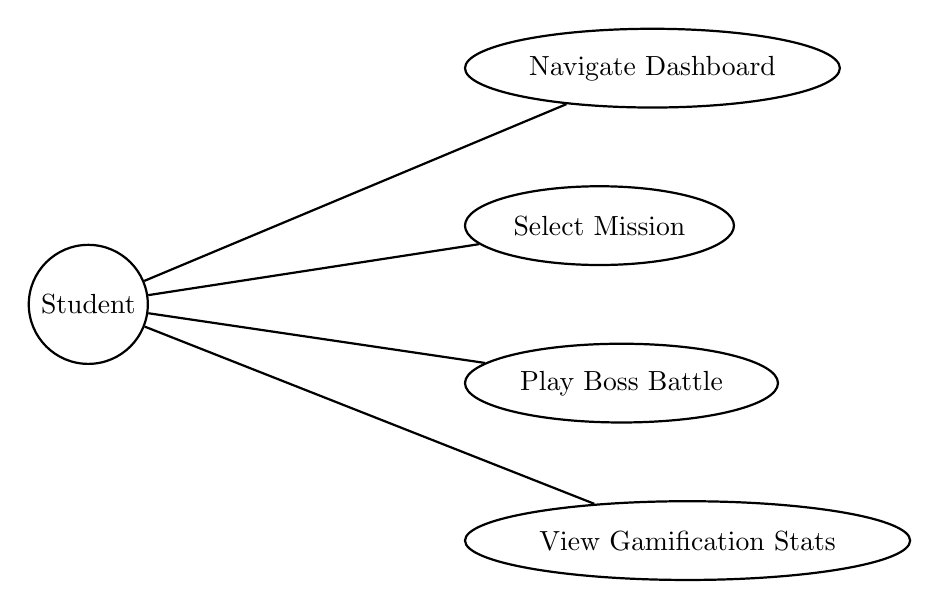
\begin{tikzpicture}[
    node distance=2.5cm,
    actor/.style={circle, draw, thick, minimum size=1.2cm, align=center},
    usecase/.style={ellipse, draw, thick, minimum width=3cm, minimum height=1cm, align=center}
]
    % Actors
    \node[actor] (student) {Student};

    % Use Cases
    \node[usecase, right=4cm of student, yshift=3cm] (uc1) {Navigate Dashboard};
    \node[usecase, right=4cm of student, yshift=1cm] (uc2) {Select Mission};
    \node[usecase, right=4cm of student, yshift=-1cm] (uc3) {Play Boss Battle};
    \node[usecase, right=4cm of student, yshift=-3cm] (uc4) {View Gamification Stats};

    % Links
    \draw[thick] (student) -- (uc1);
    \draw[thick] (student) -- (uc2);
    \draw[thick] (student) -- (uc3);
    \draw[thick] (student) -- (uc4);
\end{tikzpicture}
\end{center}
\vspace{0.5cm}

\subsection{Data Flow Diagram (Level 0 - UI Event Flow)}
This Data Flow Diagram models how user input triggers state updates within the React frontend, independent of a backend server.

\vspace{0.5cm}
\begin{center}
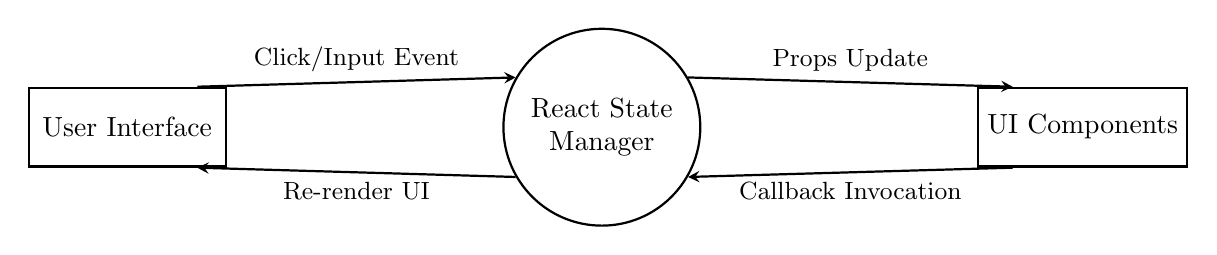
\begin{tikzpicture}[
    node distance=3cm,
    process/.style={circle, draw, thick, minimum size=2.5cm, align=center},
    entity/.style={rectangle, draw, thick, minimum width=2.5cm, minimum height=1cm, align=center},
    arrow/.style={thick,->,>=stealth}
]
    \node[entity] (user) {User Interface};
    \node[process, right=3.5cm of user] (state) {React State\\Manager};
    \node[entity, right=3.5cm of state] (component) {UI Components};

    \draw[arrow] (user.30) -- node[above] {\small Click/Input Event} (state.150);
    \draw[arrow] (state.210) -- node[below] {\small Re-render UI} (user.330);
    
    \draw[arrow] (state.30) -- node[above] {\small Props Update} (component.150);
    \draw[arrow] (component.210) -- node[below] {\small Callback Invocation} (state.330);
\end{tikzpicture}
\end{center}
\vspace{0.5cm}

\section{Software Design}

\subsection{Component Hierarchy (UML)}
The frontend is heavily componentized. The UML diagram below represents the composition of the React component tree implemented in the \texttt{src/components} directory.

\vspace{0.5cm}
\begin{center}
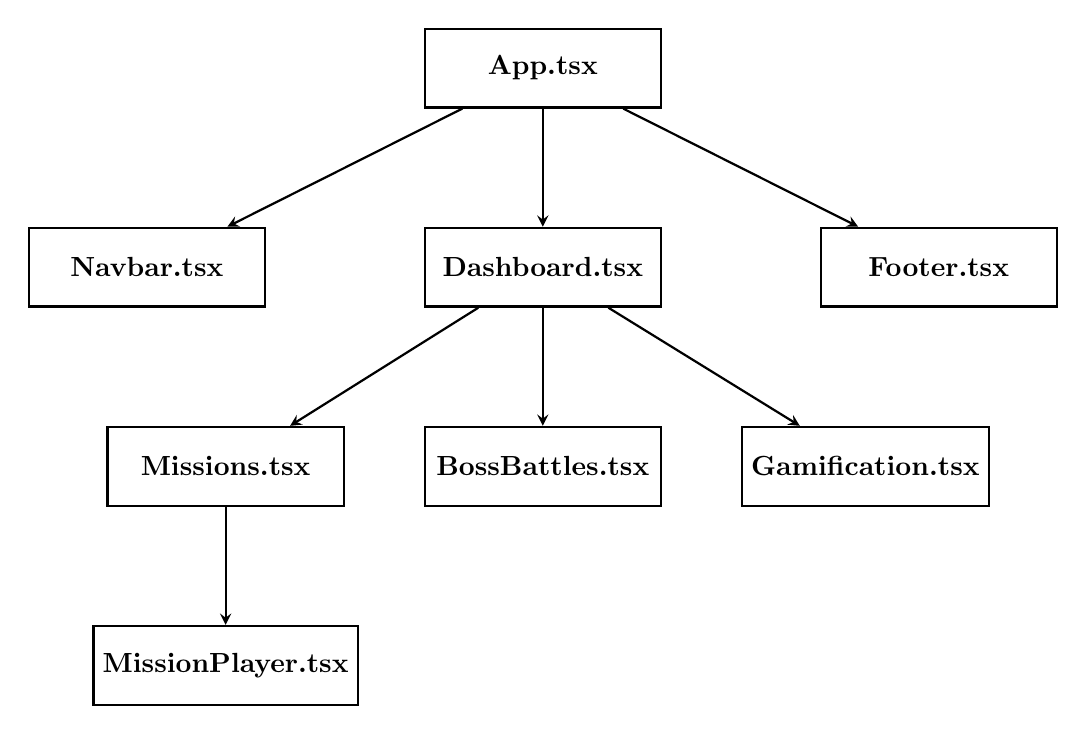
\begin{tikzpicture}[
    node distance=1.5cm,
    class/.style={rectangle, draw, thick, align=center, minimum width=3cm, minimum height=1cm}
]
    \node[class] (app) {\textbf{App.tsx}};
    
    \node[class, below left=1.5cm and 2cm of app] (nav) {\textbf{Navbar.tsx}};
    \node[class, below=1.5cm of app] (dash) {\textbf{Dashboard.tsx}};
    \node[class, below right=1.5cm and 2cm of app] (footer) {\textbf{Footer.tsx}};
    
    \node[class, below left=1.5cm and 1cm of dash] (missions) {\textbf{Missions.tsx}};
    \node[class, below=1.5cm of dash] (boss) {\textbf{BossBattles.tsx}};
    \node[class, below right=1.5cm and 1cm of dash] (gamify) {\textbf{Gamification.tsx}};
    
    \node[class, below=1.5cm of missions] (player) {\textbf{MissionPlayer.tsx}};

    \draw[-stealth, thick] (app) -- (nav);
    \draw[-stealth, thick] (app) -- (dash);
    \draw[-stealth, thick] (app) -- (footer);
    
    \draw[-stealth, thick] (dash) -- (missions);
    \draw[-stealth, thick] (dash) -- (boss);
    \draw[-stealth, thick] (dash) -- (gamify);
    
    \draw[-stealth, thick] (missions) -- (player);
\end{tikzpicture}
\end{center}
\vspace{0.5cm}

\section{Implementation Details}
The frontend implementation prioritized performance, reusability, and thematic consistency.
\begin{itemize}
    \item \textbf{\texttt{BossBattles.tsx} and \texttt{MissionPlayer.tsx}:} These are the core interactive components of the platform. They manage local state representing the user's progress through a mathematical sequence. Health bars, timer graphics, and immediate visual feedback (correct/incorrect) are handled using dynamic Tailwind CSS classes based on the component's state.
    \item \textbf{\texttt{Gamification.tsx}:} This component aggregates the user's virtual currency (Spider Points), unlocked badges, and current tier. It leverages animated progress bars to visually represent proximity to the next level.
    \item \textbf{\texttt{useGameState.ts}:} A custom React hook implemented to abstract complex game logic (e.g., score calculation, combo multipliers, health point tracking) away from the presentation components, ensuring the UI code remains clean and maintainable.
\end{itemize}

\chapter{Results and Evaluation}

\section{Testing Methodology}
As the project is currently in the frontend prototype stage, testing was focused on Component Verification and UI/UX validation rather than backend integration.
\begin{itemize}
    \item \textbf{Component Testing:} Manual isolated testing of interactive elements (e.g., verifying that submitting an answer in \texttt{MissionPlayer.tsx} correctly updates the local score state).
    \item \textbf{Responsiveness Testing:} Verifying that the Tailwind CSS layouts scale correctly across mobile, tablet, and desktop viewports.
    \item \textbf{Performance Auditing:} Utilizing Vite's build tools to ensure bundle sizes remain small and utilizing Lighthouse to verify rapid "First Contentful Paint" times.
\end{itemize}

\section{System Verification}

\begin{table}[h]
\centering
\begin{tabular}{@{}p{3.5cm}p{8.5cm}l@{}}
\toprule
\textbf{Component / Flow} & \textbf{Verified Behaviour} & \textbf{Result} \\ \midrule
Responsive Layout & \texttt{Navbar.tsx} and \texttt{Hero.tsx} stack correctly on mobile screens. & Pass \\ 
Mission Selection & Clicking a mission dynamically mounts the \texttt{MissionPlayer.tsx} component. & Pass \\ 
Game State Hook & \texttt{useGameState.ts} accurately increments score upon correct simulated input. & Pass \\ 
Thematic Styling & Custom Tailwind configuration successfully applies global fonts and hero-colors. & Pass \\ \bottomrule
\end{tabular}
\caption{Summary of frontend functional verification}
\end{table}

\section{Analysis}
The frontend prototype successfully establishes the visual and interactive foundation for MathVerse AI. The use of Vite and React provided a highly productive developer experience, resulting in a fast, robust SPA. The modular component architecture ensures that when the backend REST API is introduced, data fetching can be easily integrated into the existing higher-order components (like \texttt{Dashboard.tsx}) and passed down as props without requiring a complete rewrite of the UI logic.

\chapter{Conclusion}

\section{Summary of Work}
During this phase, the complete presentation layer of MathVerse AI was designed and implemented. A cohesive, superhero-themed user interface was built using React and Tailwind CSS, featuring over 12 distinct interactive components. Client-side state management was established to simulate the gamified mathematical learning experience.

\section{Key Findings}
\begin{itemize}
    \item \textbf{Component Modularity is Critical:} Separating the UI into distinct components (\texttt{Missions.tsx}, \texttt{BossBattles.tsx}) made managing the complex gamified UI significantly easier.
    \item \textbf{Custom Hooks Simplify UI:} Abstracting the game logic into \texttt{useGameState.ts} kept the presentation components declarative and easy to read.
    \item \textbf{Tailwind CSS Accelerates Prototyping:} The utility-first approach allowed for rapid iteration of the platform's unique superhero aesthetic without managing complex CSS files.
\end{itemize}

\section{Future Work and Recommendations}
\begin{enumerate}
    \item \textbf{Backend API Integration:} Connect the frontend to the Node.js/Python backend to fetch live user data, mission parameters, and persist gamification state to PostgreSQL.
    \item \textbf{AI Problem Fetching:} Replace the static/mocked math problems in \texttt{MissionPlayer.tsx} with dynamically generated JSON payloads from the LLM service.
    \item \textbf{Authentication Integration:} Implement JWT verification on the frontend and wrap the \texttt{Dashboard.tsx} in a protected route component.
    \item \textbf{Advanced Animations:} Integrate Framer Motion to add more sophisticated entry and exit animations during Boss Battles for a highly polished experience.
\end{enumerate}

\section{Final Remarks}
The completed frontend prototype proves the viability of the MathVerse AI concept. By securing a highly engaging, responsive user interface first, the project is perfectly positioned for the next phase: integrating the AI generation pipeline and persistent database architectures.

\end{document}
